%%%%%%%%%%%%%%%%%%%%%%%%%%%%%%%%%%%%%%%%%
% Stylish Article
% LaTeX Template
% Version 2.1 (1/10/15)
%
% This template has been downloaded from:
% http://www.LaTeXTemplates.com
%
% Original author:
% Mathias Legrand (legrand.mathias@gmail.com) 
% With extensive modifications by:
% Vel (vel@latextemplates.com)
%
% License:
% CC BY-NC-SA 3.0 (http://creativecommons.org/licenses/by-nc-sa/3.0/)
%
%%%%%%%%%%%%%%%%%%%%%%%%%%%%%%%%%%%%%%%%%

%----------------------------------------------------------------------------------------
%	PACKAGES AND OTHER DOCUMENT CONFIGURATIONS
%----------------------------------------------------------------------------------------

\documentclass[fleqn,12pt]{SelfArx_ch} % Document font size and equations flushed left

\usepackage[english]{babel} % Specify a different language here - english by default

\usepackage{lipsum} % Required to insert dummy text. To be removed otherwise

\captionsetup[figure]{justification=justified, singlelinecheck=off} 
\captionsetup[table]{justification=justified, singlelinecheck=off} 

%----------------------------------------------------------------------------------------
%	COLUMNS
%----------------------------------------------------------------------------------------

\setlength{\columnsep}{0.55cm} % Distance between the two columns of text
\setlength{\fboxrule}{0.75pt} % Width of the border around the abstract
\linespread{1.5}

%----------------------------------------------------------------------------------------
%	COLORS
%----------------------------------------------------------------------------------------

\definecolor{color1}{RGB}{0,0,90} % Color of the article title and sections
\definecolor{color2}{RGB}{10,20,20} % Color of the boxes behind the abstract and headings
\definecolor{xsubj}{RGB}{243,194,68} 
\definecolor{xsess}{RGB}{53,99,161} 
\definecolor{xsamp}{RGB}{18,165,121} 

%----------------------------------------------------------------------------------------
%	HYPERLINKS
%----------------------------------------------------------------------------------------

\usepackage{hyperref} % Required for hyperlinks
\hypersetup{hidelinks,colorlinks=true,breaklinks=true,urlcolor=color1,citecolor=color1,linkcolor=color1,bookmarksopen=false,pdftitle={Title},pdfauthor={Author}}
%----------------------------------------------------------------------------------------
%	ARTICLE INFORMATION
%----------------------------------------------------------------------------------------

% \JournalInfo{Journal, Vol. XXI, No. 1, 1-5, 2013} % Journal information
\JournalInfo{Frontiers in Neuroinformatics}
\DOI{https://doi.org/10.3389/fninf.2019.00012}
\Archive{ }
\PaperTitle{Ch.I: A Serverless Tool for Platform Agnostic Computational Experiment Management}
\Authors{Gregory Kiar\textsuperscript{1}, Shawn T. Brown\textsuperscript{1}, Tristan Glatard\textsuperscript{2},
Alan C. Evans\textsuperscript{1}} % Authors
\affiliation{\textsuperscript{1}\textit{Montréal Neurological Institute, McGill University, Montréal, QC, Canada}}
\affiliation{\textsuperscript{2}\textit{Department of Computer Science and Software Engineering, Concordia University, Montréal, QC, Canada}}
%----------------------------------------------------------------------------------------
%	ABSTRACT
%----------------------------------------------------------------------------------------

\Abstract{Neuroscience has been carried into the domain of big data and high performance computing (HPC) on the backs
of initiatives in data collection and an increasingly compute-intensive tools. While managing HPC experiments requires
considerable technical acumen, platforms, and standards have been developed to ease this burden on scientists. While
web-portals make resources widely accessible, data organizations such as the Brain Imaging Data Structure and tool
description languages such as Boutiques provide researchers with a foothold to tackle these problems using their own
datasets, pipelines, and environments. While these standards lower the barrier to adoption of HPC and cloud systems for
neuroscience applications, they still require the consolidation of disparate domain-specific knowledge. We present
Clowdr, a lightweight tool to launch experiments on HPC systems and clouds, record rich execution records, and enable
the accessible sharing and re-launch of experimental summaries and results. Clowdr uniquely sits between web platforms
and bare-metal applications for experiment management by preserving the flexibility of do-it-yourself solutions while
providing a low barrier for developing, deploying and disseminating neuroscientific analysis.}

%----------------------------------------------------------------------------------------

\begin{document}
\flushbottom % Makes all text pages the same height
\maketitle % Print the title and abstract box
\thispagestyle{empty} % Removes page numbering from the first page
\clearpage
\makeabstract

\onecolumn 
\beginchapter{I}
%----------------------------------------------------------------------------------------
%	ARTICLE CONTENTS
%----------------------------------------------------------------------------------------
\section{Introduction}
The increasing adoption of distributed computing, including cloud and high-performance computing (HPC), has played a
crucial role in the expansive growth of neuroscience. With an emphasis on big-data analytics, collecting large datasets
such as the Consortium for Reliability and Reproducibility~\cite{Zuo2014-sj}, UK-Biobank~\cite{Sudlow2015-dl}, and
Human Connectome Project~\cite{Van_Essen2013-bx} is becoming increasingly popular and necessary. While these datasets
provide the opportunity for unprecedented insight into human brain function, their size makes non-automated analysis
impractical.

At the backbone of science is the necessity that claims are reproducible. The reproducibility of findings has entered
the spotlight as a key question of interest, and has been explored extensively in
psychology~\cite{Open_Science_Collaboration2015-ja}, neuroimaging~\cite{bowring2019exploring,Eklund2016-wo}, and other
domains~\cite{Baker2016-en,Milkowski2018-je}. Computational experiments must be re-executable as a critical condition
for reproducibility, and this bare minimum requirement becomes increasingly challenging with larger datasets and more
complex analyses. While sharing all code and data involved may appear a compelling solution, this is often inadequate
for achieving re-runnability or reproducibility of the presented findings and models~\cite{Milkowski2018-je}. When
re-executable applications fail to reproduce findings, there is a gray area where the source of errors are often
unknown and may be linked to misinterpretation of data, computing resources or undocumented execution details, rather
than scientific meaning.

As a result, new tools and standards have emerged to aid in producing more reusable datasets and tools, and thereby
more reproducible science. The Brain Imaging Data Structure (BIDS)~\cite{Gorgolewski2016-om} and the associated BIDS
apps~\cite{Gorgolewski2017-sr} prescribe a standard for sharing and accessing datasets, and therefore, increasing the
accessibility and impact of both datasets and tools. This standard includes the definition of file organization on
disk, as well as key-value pairs of metadata information in JavaScript Object Notation (JSON) files, and assigns
specific meaning to command-line arguments to be used when processing these datasets. The Boutiques
framework~\cite{Glatard2018-uw} provides a standard for software documentation in a machine-interpretable way, allowing
the automation of tool execution and evaluation. These descriptions fully encapsulate the runtime instructions for a
given tool in JSON-files, and are appropriate for a majority of command-line applications. Software containerization
initiatives such as Docker~\cite{Merkel2014-vu} and Singularity~\cite{Kurtzer2017-kq} facilitate execution consistently
across arbitrary computing environments with minimal burden on the user.

Web-platforms such as OpenNeuro~\cite{Poldrack2013-wi}, LONI Pipeline~\cite{Rex2003-pr}, and
CBRAIN~\cite{Sherif2014-ve} simplify the analysis process further by providing an accessible way to construct
neuroscience experiments on commonly used tools and uploaded-datasets. These systems deploy tools on HPC environments
and record detailed execution information so that scientists can keep accurate records and debug their workflows. Tools
such as LONI’s provenance manager~\cite{Dinov2010-yq}, Reprozip~\cite{Chirigati2016-ep}, and ReCAP~\cite{Hasham2018-hn}
capture system-level properties such as system resources consumed and files accessed, where tools supporting the
Neuroimaging Data Model (NIDM)~\cite{Sochat2016-gl}, a neuroimaging-specific provenance model based on
W3C-PROV~\cite{Missier2013-ml}, capture information about the domain-specific transformations applied to the data of
interest.

The initiatives enumerated above have synergistic relationships, where each solves a small but significant piece of the
larger puzzle that is computational and scientific reproducibility and replicability. However, the learning curve
associated with adopting each of these technologies is considerable, leveraging them in an impactful way is difficult,
and certain applications may benefit from different approaches so these learning curves may have to be paid multiple
times. For instance, interoperability is mainly valuable in contexts which there is a large variety of datasets or
tools, and provenance may be of importance to identify the impact of an underlying system on a processing or modeling
task. We present Clowdr, a lightweight tool which ties these approaches together so that researchers can minimize the
learning burden and lower the barrier to develop, perform, and disseminate reproducible, interoperable and
provenance-rich neuroscience experiments.

\section{Emergent Technologies in Reproducible Neuroscience}

Conducting reproducible analyses in neuroscience requires many complementary facets, building on technologies which are
commonly adopted as \textit{de facto} standards.

\subsection{Data and Code Interoperability}
Due in part to its simplicity and active public development community, BIDS~\cite{Gorgolewski2016-om} has become an
increasingly prominent data organization format in neuroimaging. This standard makes use of the Nifti file
format~\cite{Cox2004-qw} and human-readable JSON files to capture both imaging and subject-specific metadata. An
important benefit of this data organization is the ability to launch data processing pipelines in the form of BIDS
applications~\cite{Gorgolewski2017-sr}, which expose a consistent set of instructions compatible with the data
organization. Together, these complementary standards are suitable for performing a large variety of neuroimaging
experiments. In contexts where tools have heterogeneous interfaces, or data organizations are custom-built for a
particular context, the Boutiques~\cite{Glatard2018-uw} framework allows the rich description of a pipeline such that
tool execution, validation, and exploration can be automated. These descriptors include the command-line structure to
be populated as well as rich parameter descriptions and interactions, such as mutually exclusivity or dependence, such
that complicated data interactions required or forbidden by the tool can be accounted for.

\subsection{Software Virtualization}
While virtual machines have long been used for deploying analysis pipelines with complex dependencies in heterogeneous
environments, software containers have recently emerged as lighter-weight alternatives suitable for transient data
processing applications. Docker~\cite{Merkel2014-vu} provides this functionality across all major host operating
systems, but is often not supported by HPC centers due to security vulnerabilities~\cite{Bui2015-pd,Combe2016-vb}.
Singularity~\cite{Kurtzer2017-kq} addresses the security risks of Docker, but currently only supports Linux operating
systems, filling the niche of containerization on shared computing resources. A detailed comparison in the context of
medical imaging can be found in~\cite{Matelsky2018-sy}.

\subsection{Workflow Engines}
Custom scientific pipelines can be composed in Python with Nipype~\cite{Gorgolewski2011-pq},
Dask~\cite{Rocklin2015-na}, Pegasus~\cite{Deelman2015-ui}, Toil~\cite{Vivian2017-ul}, or several other tools which
facilitate the modular interaction of complex independent processing stages. While the underlying tasks in Nipype,
Dask, and Toil are defined in Python, Pegasus uses a Domain Specific Language (DSL) for representing tasks, increasing
the barrier for defining tasks but ultimately increasing their portability. While Nipype is a widely used tool in
neuroimaging and has many readily-defined interfaces available for researchers, the others require non-insignificant
development to describe interfaces for common neuroimaging applications such as FSL~\cite{Jenkinson2012-ly} or
MRtrix~\cite{Tournier2012-po}. PSOM~\cite{Bellec2012-um} and Scipipe~\cite{Lampa2018-xn} are functionally similar to
Nipype but have been developed for GNU Octave/MATLAB and Golang, respectively. Several domains have more specialized
tools which accomplish similar feats in their area of interest. These include Pypet~\cite{Meyer2016-zt},
Neuromanager~\cite{Stockton2015-ex}, Arachne~\cite{Aleksin2017-ms}, and others which facilitate the automation of
modeling and simulation workflows using tools such as Neuron~\cite{Hines2001-wo}. For an in depth look at other tools
in this space please refer to~\cite{Meyer2016-zt} and~\cite{Stockton2015-ex}. Each of these tools enables the
construction of dependency graphs between pipeline components, and allow the deployment either to cluster scheduling
software, multiple processing threads, and in some cases computing clouds. These tools primarily function through
programmatic interfaces, though LONI pipeline~\cite{Rex2003-pr}, OpenMOLE~\cite{Reuillon2013-zo}, and
Galaxy~\cite{Goecks2010-cl} provide both DSL and graphical user interfaces. Many of these tools also embed provenance
capture, fault-tolerance features, and data tracking to avoid recomputations across similar executions. While each of
these tools is a powerful and attractive option for creating workflows, they remain complex and potentially overkill
when launching atomic single-step analyses, prebuilt pipelines, or analysis software developed in a different language
than the workflow engine of choice.

\subsection{Provenance}
Building on the W3-PROV~\cite{Missier2013-ml} standard for data provenance metadata put forth by the World Wide Web
Consortium, NIDM~\cite{Sochat2016-gl} is a standard which represents a processing and data provenance graph specific to
neuroimaging analyses. While this standard is machine-interpretable and interoperable-by-design, supporting it
currently requires tight integration with analysis pipelines. In LONI pipeline, a provenance model exists which
includes detailed records of data use and file lifecycle~\cite{Dinov2010-yq}, which is designed to inform data
consumers what types of analyses can be and have been performed with the data in question; this tool is tightly coupled
with the LONI pipeline ecosystem. The ReCAP~\cite{Hasham2018-hn} project has been developed to evaluate the resource
consumption of arbitrary pipelines on the cloud and can aid in cloud-instance optimization. While this tool has
potential for a large impact in designing both cost effective and scalable analyses, there is considerable overhead as
it manages executions through a persistent server and workflow engine. While various other libraries exist to monitor
some piece of data or compute provenance, Reprozip~\cite{Chirigati2016-ep} is perhaps the most exciting as it uniquely
captures records of all files accessed and created throughout an execution, which allows for the creation of rich file
dependency graphs. The limitation of this technique is that it requires data of interest to be written to disk, as
opposed to managed in memory, which may not always be the case in some applications.

\subsection{Web Platforms}
Increasing the portability and accessibility of launching large scale analyses, web platforms such as
CBRAIN~\cite{Sherif2014-ve}, LONI pipeline~\cite{Rex2003-pr}, and OpenNeuro~\cite{Poldrack2013-wi} provide
science-as-a-service where users can upload and process their data on distant computing resources. Additionally, these
platforms provide an accessible and immediate way to share the results produced from experiments with collaborators or
the public. These tools provide incredible value to the community and allow the deployment of production-level
pipelines from the web, but they are not suitable for prototyping analyses or developing pipelines, and it is
cumbersome to run these services on a lab’s own resources. In addition, monolithic Web interfaces are only suitable for
a certain type of use-cases and high-level users, while developers or computer-savvy users prefer to rely on modular
command-line tools and libraries.

\clearpage
\section{The Clowdr Microtool}

\begin{figure*}[h!]
\centering
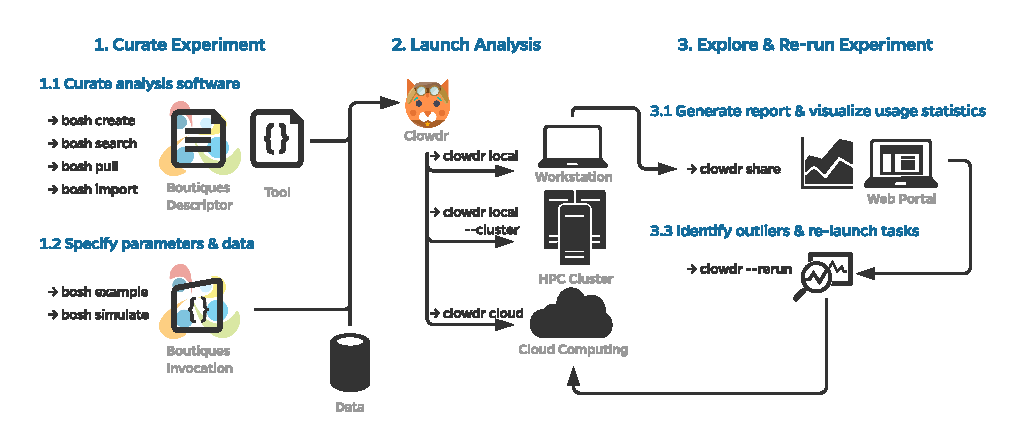
\includegraphics[width=\textwidth]{./figures/fig1.pdf}
\caption{Clowdr Workflow. \textbf{(1)} Prior to launching an analysis with Clowdr, users must curate the
analysis tools and their inputs. For the sake of portability, Clowdr supports both native and containerized
applications described in the Boutiques format. Several tools exist in Boutiques which simplify the adoption/creation
or execution of tools and are enumerated in (\textbf{1.1},\textbf{1.2}), respectively. \textbf{(2)} Scientists can then
launch their analysis with Clowdr either locally, on HPC systems, or computing clouds. Possible workflows could involve
the tuning of hyperparameters locally on a subset of the dataset of interest, and ultimately deploying the analysis at
scale using the same arguments, or sweeping hyperparameter values on an HPC system. \textbf{(3)} After execution,
summary reports can be produced by Clowdr \textbf{(3.1)} and visualized through a custom web portal enabling filtering
by both execution properties and parameters, facilitating outlier detection and comparison across executions.
Identified outliers, such as failures, incomplete tasks, or those which consumed more resources than expected can be
re-run through Clowdr without having to regenerate any of the information previously provided. Clowdr facilitates the
development, deployment, and debugging of analyses in a closed-loop provenance-rich microservice.}
\label{fig:ch1.1}
\end{figure*}
While the technologies enumerated above are essential pieces toward reproducible neuroscience, they are largely
isolated from one another and place a large burden on researchers who wish to adopt all of these best practices. Clowdr
leverages these tools to increase the deployability, provenance capture, and shareability of experiments. In summary,
Clowdr:

\begin{enumerate}[label=\roman*]
\item is tightly based on Boutiques and is BIDS-aware, supporting both arbitrary pipelines and providing an accessible
entrypoint for neuroimaging;
\item executes both bare-metal workflows and Docker or Singularity virtualized pipelines through Boutiques on local,
HPC, and cloud resources;
\item supports the parallelized batch deployment and redeployment of pipelines constructed with workflow-engines, while
being agnostic to programming language and construct;
\item captures system-level provenance information (i.e., CPU and RAM usage), supports Reprozip, and internal
provenance captured by arbitrary pipelines such as NIDM; and
\item supports the deployment of both development- and production-level tools without an active server, and provides a
web-report for exploring and sharing experiments.
\end{enumerate}

A typical workflow using Clowdr is summarized in Figure~\ref{fig:ch1.1}. While a Clowdr experiment follows the same
workflow as traditional experiments, beginning with tool and data curation through prototyping, deployment, and
exploration, there are several considerable benefits provided by Clowdr over traditional approaches. In particular,
Clowdr is based on the rich Boutiques framework for tool description and execution, ensuring that documentation,
parameter definitions, and real-world parameter values accompany the tool at all times. Clowdr also treats all
computing systems the same, from the users perspective, so transitioning from local development of analyses to at-scale
systems is seamless, which minimizes errors made during this transition. Clowdr also provides a visualization portal
for exploring executions and filtering either based on parameter values or runtime statistics, allowing for quality
control of the execution in addition to commonly used quality control of processed derivatives themselves.

Figure~\ref{fig:ch1.2} shows the execution lifecycle within Clowdr. Starting from user-provided Boutiques descriptor
(B) and invocation(s) (C), and access to any required datasets, Clowdr begins by identifying a list of tasks to launch.
For a new experiment, tasks are identified in one of three main ways: (1) a one:one mapping from a list of invocations,
(2) a one:many mapping from a single invocation in which parameter(s) have been specified for sweeping during
execution, or a BIDS-specific, and (3) one:many mapping from a single invocation for a BIDS app, which will iterate
upon the participant- and session-label fields, and described in the BIDS app specification~\cite{Gorgolewski2017-sr}.
Experiments can be re-run, and determine the task-list based on whether a full, failure-only, or incomplete-only
re-execution is desired. Once the task-list is determined, Clowdr creates an independent invocation which explicitly
defines the arguments used in each task.

\begin{figure*}[h!]
\centering
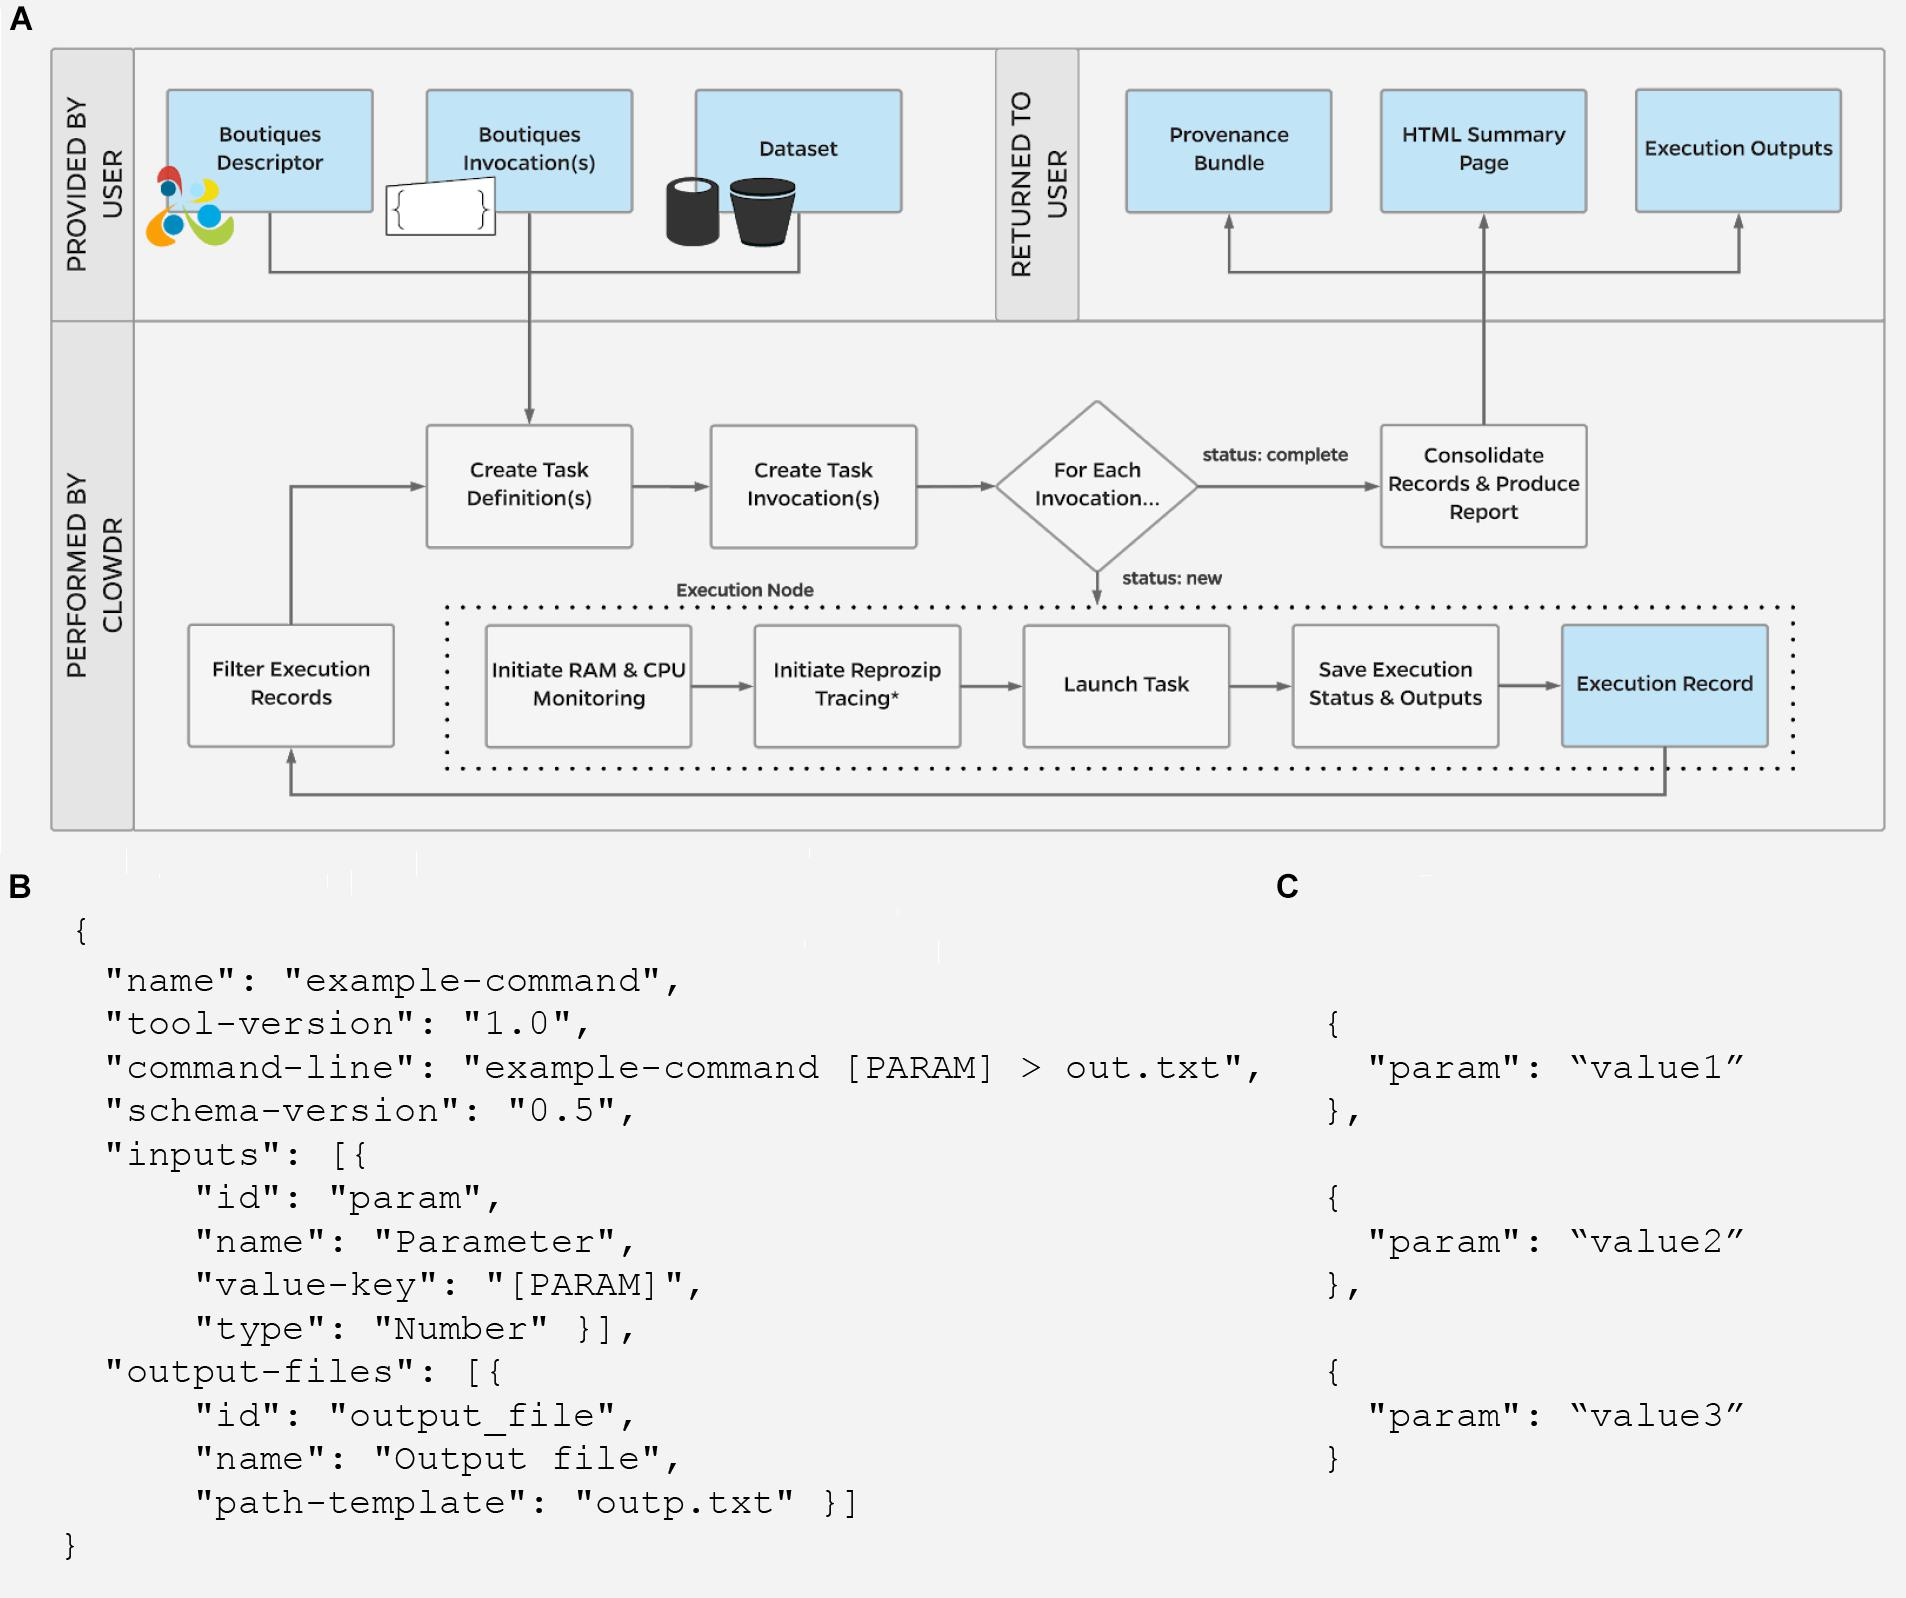
\includegraphics[width=0.95\textwidth]{./figures/fig2.jpg}
\caption{\textbf{(A)} Clowdr Data Flow. Beginning with a user-supplied tool descriptor \textbf{(B)} and parameter
invocation(s) \textbf{(C)}, Clowdr identifies unique tasks to launch and wraps each with usage and log monitoring
tools, to ultimately provide a rich record of execution to the user alongside the expected output products of the
experiment. Clowdr ultimately produces an HTML summary for users to explore, update, filter, and share the record of
their experiment. In the above schematic, blue boxes indicate data, where gray indicate processing steps. *External
reprozip tracing is supported on limited infrastructures, as running virtualized environments within a trace capture
requires elevated privileges which may be a security risk on some systems.}
\label{fig:ch1.2}
\end{figure*}

At this stage, Clowdr distributes tasks to the Cloud system or local cluster scheduler being used for deployment.
Presently Clowdr supports the SLURM scheduler and Amazon Web Services (AWS) cloud through their Batch service with
adoption of more platforms ongoing. Each task is launched through a Clowdr-wrapper, which initializes CPU and RAM
monitoring and triggers Reprozip tracing prior to launching the analysis itself. Reprozip tracing has limited support
in conjunction with containerized analyses on HPC systems due to potential security issues. Reprozip is built upon the
Linux command “ptrace,” which traces processes to monitor or control them. To eliminate the potential risk of using
this tool, it is common for systems to disallow the tracing of administrator-level processes. The requirement of
limited administrator privileges by Singularity (during the creation of multiple user namespaces) and Docker (for
interacting with the daemon) makes encapsulating these tools within the restricted ptrace scope not possible on many
shared systems. For more information on the specific conditions in which these technologies can be made to interoperate
please view the GitHub repository for this manuscript, linked below.

\begin{figure*}[p!]
\centering
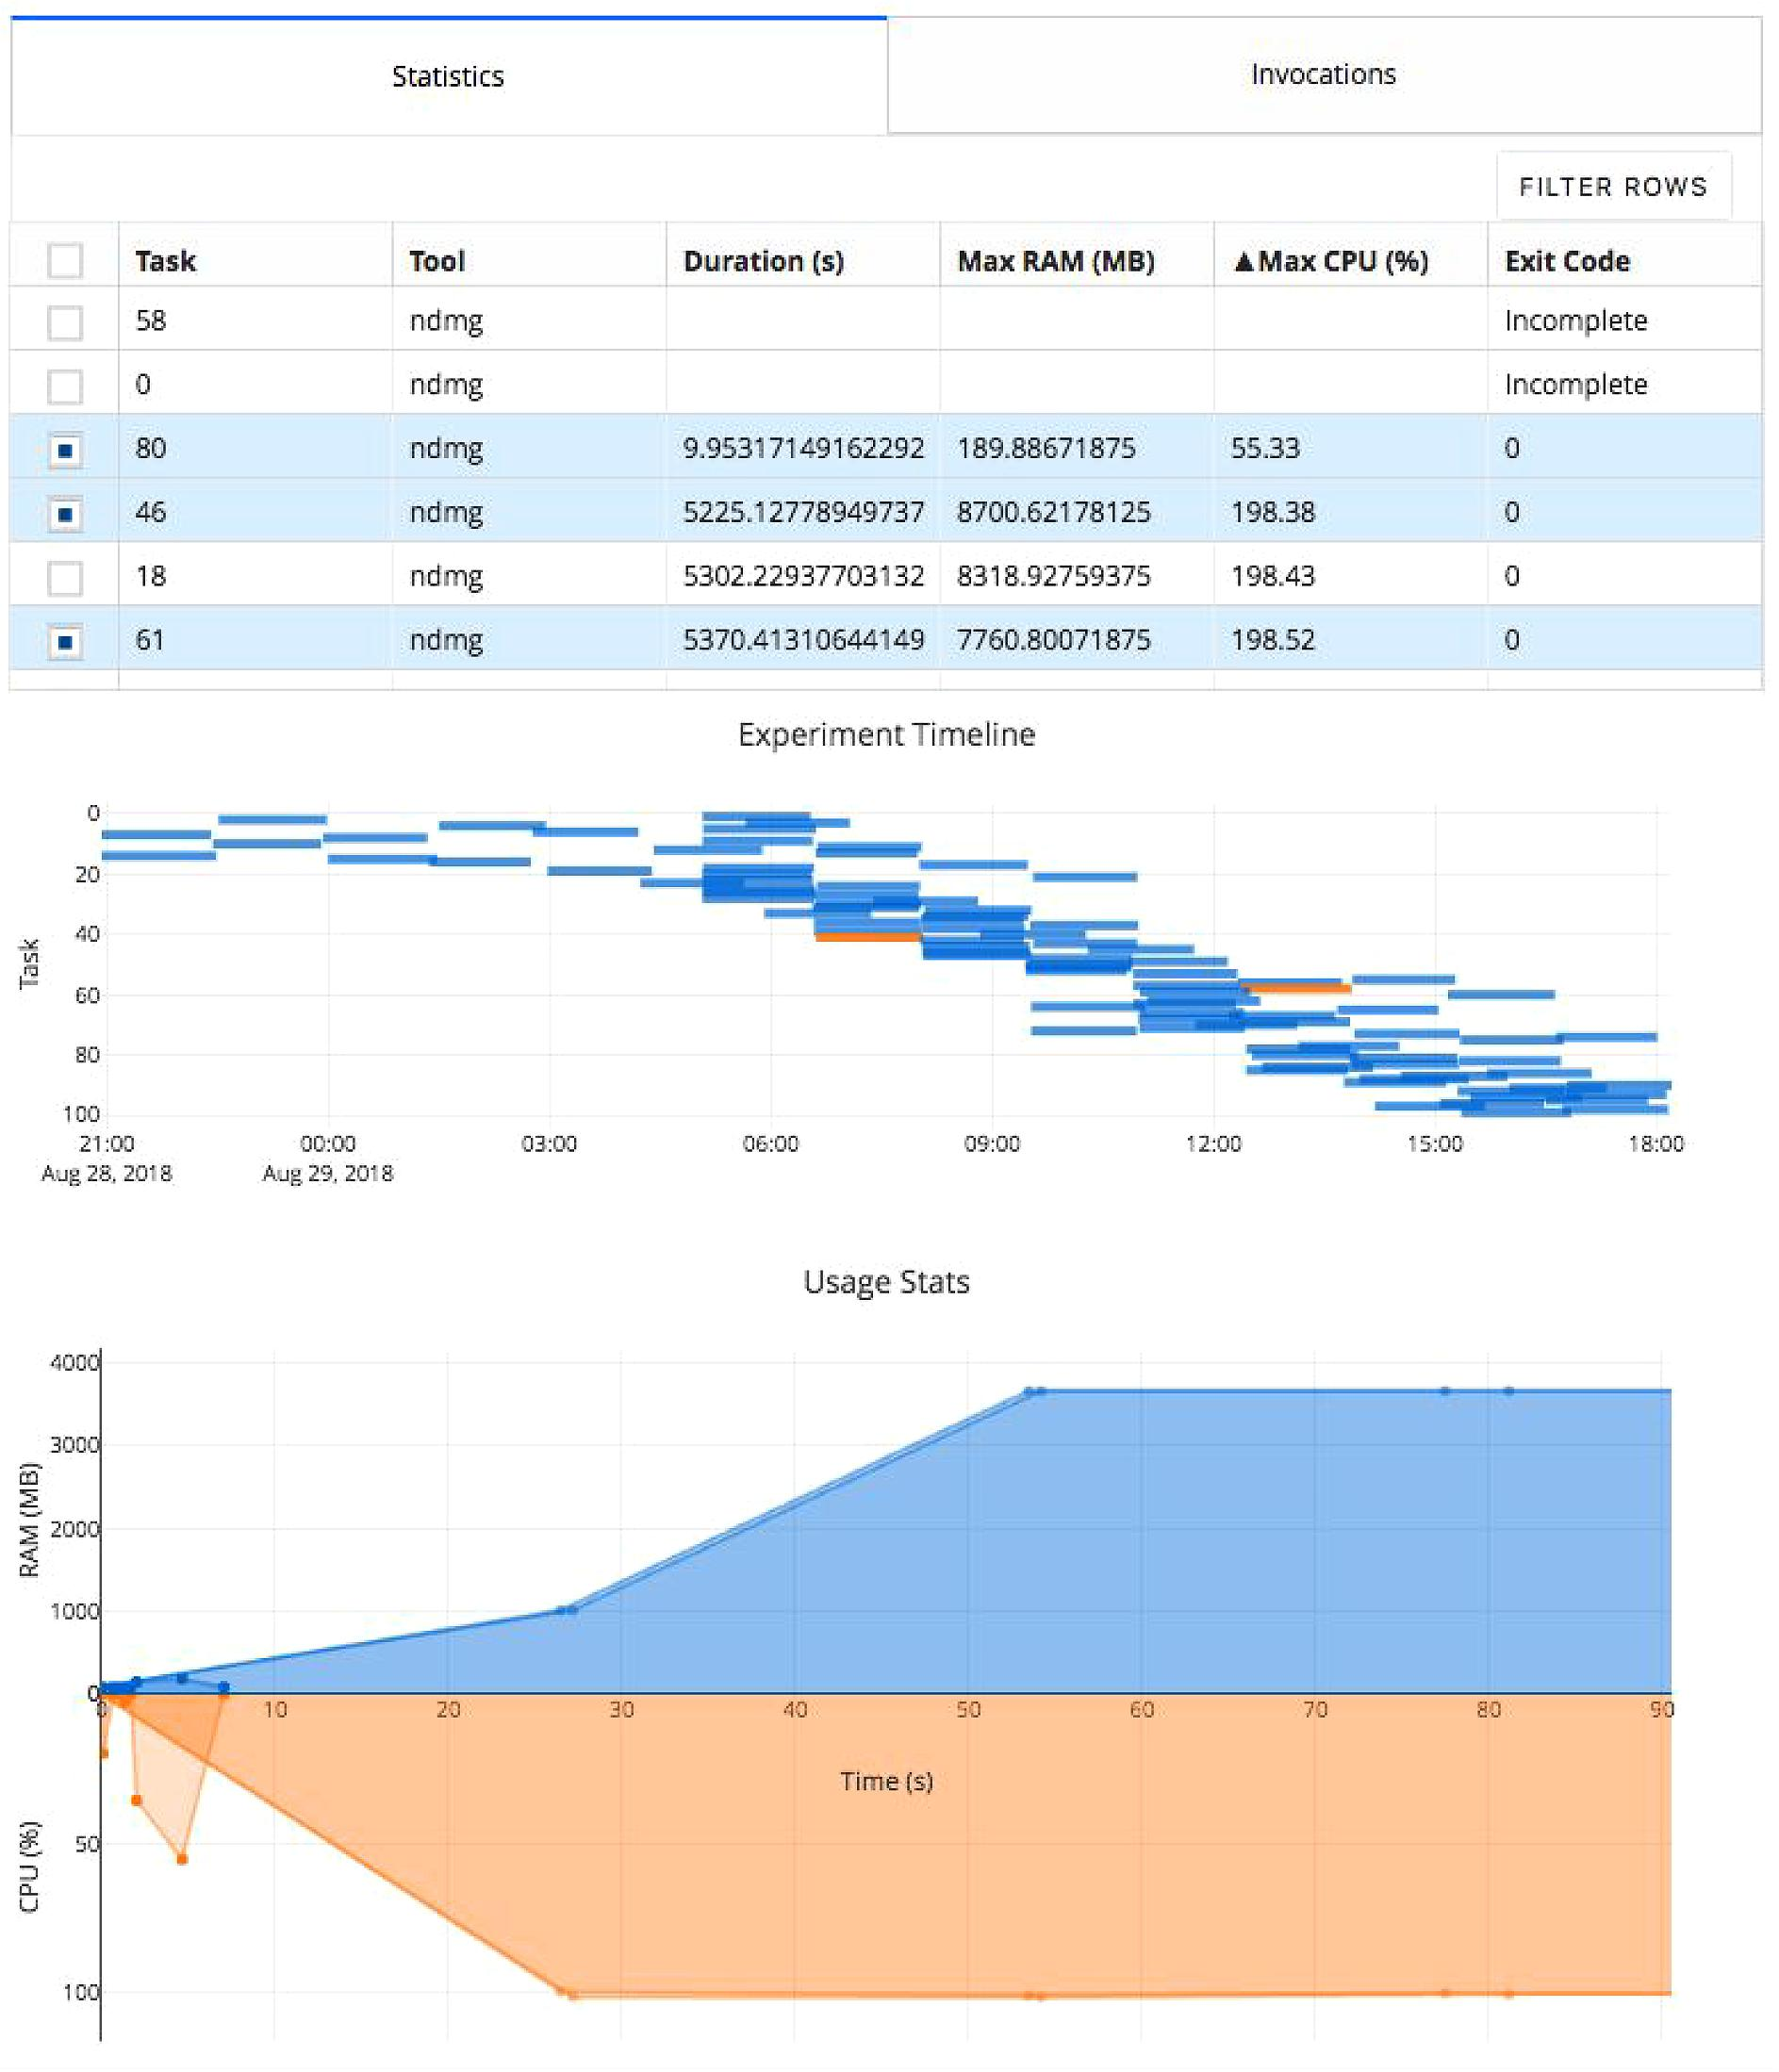
\includegraphics[width=0.7\textwidth]{./figures/fig3.jpg}
\caption{Clowdr Experiment Viewer. Experiments launched with Clowdr can be monitored and both progress and runtime
statistics explored. The page is produced using Plotly Dash to produce highly interactive plots and tables, enabling
rich filtering, rescaling, and exploration of executions. The table can be toggled to present summary statistics about
experiment execution or invocation parameters identifying parameters used for each task in the experiment. The
subsequent Gantt plot shows the timeline of executed tasks in the experiment, where those selected for visualization in
the usage plot below are highlighted. The final plot in this view shows the memory and processing footprint throughout
all selected tasks. Selection and filtering may be done by value in the tables or selection in the task timeline. In
this example, several tasks did not complete and one appeared to exit after 10 s erroneously. The Clowdr portal enables
quick identification of these outliers, and the table view can be switched to identify more information such as
parameters pertaining to the executions of interest. For more information about the pipeline being executed in
particular, please see~\cite{Kiar2018-lz}.}
\label{fig:ch1.3}
\end{figure*}

Upon completion of the analysis, Clowdr bundles the system monitored records, standard output and error, exit status,
and any other information collected by either the tool itself or the Boutiques runtime engine, and concludes its
execution. Once the experiment has begun, Clowdr provides the user with the Clowdr provenance directory which will be
updated automatically as executions progress.

The researcher can monitor the provenance directory using the Clowdr share portal (Figure~\ref{fig:ch1.3}), which
provides a web interface summarizing the task executions. Once the analysis concludes, the figures on this web page and
the associated metadata can be saved and serve as a record of the experiment either for evaluation or dissemination
alongside published results.

The Clowdr package is open-source on GitHub~\cite{Kiar2018-lq}, and installable through the Python Package Index.

\section{Performing Experiments With Clowdr}

Here, we explore an experiment in which we used Clowdr to process the Human Connectome Project
(HCP)~\cite{Van_Essen2013-bx} dataset with a structural and functional connectome estimation pipeline,
ndmg~\cite{Kiar2018-lz}. The records of this experiment, and materials and instructions that can be used to reproduce a
similar analysis with Clowdr using the publicly available DS114 BIDS dataset~\cite{Poldrack2013-wi} an the example BIDS
application~\cite{Gorgolewski2017-sr} can be found on Github at: \url{https://github.com/clowdr/clowdr-paper}. Specific
packages and their versions for both experiments can be found at the end of this manuscript.

As summarized above, performing an analysis with Clowdr requires the creation of a Boutiques descriptor summarizing the
pipeline of interest, an invocation containing the parameters to supply to this pipeline on execution, and curation of
the data to be processed. There are several utilities in Boutiques which aid in this setup process, including to
automatically generate a descriptor and sample inputs from a tool, and can be explored in the associated
documentation~\cite{Glatard2018-uw}.

Clowdr experiments can be launched locally, on cluster, or submitted to cloud resources. In each case, invocations and
task definitions are created locally, and then the jobs are run serially, submitted to a cluster queue, or pushed to
cloud storage and called remotely. The commands used in Clowdr to launch these commands are the local, local with the
cluster switch, and cloud modes, respectively. Upon completion of each tasks, summary files created by Clowdr can be
either inspected manually or consolidated and visualized in the web with the Clowdr share command
(Figure~\ref{fig:ch1.3}).

The share tool, launchable on any computer with access to the experiment, creates a lightweight web service displaying
summary statistics and invocation information from the experiment, including memory usage, task duration, launch order,
and log information. The visualizations provided are filterable and sortable, enabling users to interrogate and
identify outliers in their experiment, explore potential sources of failure, and effectively profile the analysis
pipeline in use. The modified figures can be downloaded from this interface, serving as accessible records of
execution.

In the example above, the HCP dataset has been processed using a pipeline performing image denoising, registration,
model fitting, and connectivity estimation, all of which are commonly used processing steps in neuroimaging. For more
information on this pipeline, please see~\cite{Kiar2018-lz}.

In this experiment the table has been filtered to show several tasks which appeared spurious in their execution
compared to the others. We can see that several tasks failed to complete and one appeared to terminate in significantly
less time than the others. After identifying these tasks and exploring the time series’ to see at what stage of
processing the job failed (in this case, immediately), we can investigate parameter selections used in each and attempt
the re-execution of these jobs using the local or cloud command with the rerun switch in Clowdr. Clowdr provides a
layer of quality control on executions, in addition to that which is regularly performed by researchers on their
datasets, which provides immediate value when identifying task failures which otherwise may be difficult to identify,
especially in cases which intermediate and terminal derivatives are written to the same location, which can often be
the case with transformations estimated by registration pipelines, for example.

While the share tool currently requires maintaining an active server, the plots can be exported statically and it is in
the development roadmap to enable exporting the entire web page as static files, as discussed here:
\url{https://github.com/plotly/dash/issues/266}. Since the record created by Clowdr is stored in the machine-readable
and JSON format, researchers can easily extract their records and integrate it into other interfaces that suit their
application.

\section{Discussion}
Clowdr addresses several barriers to performing reproducible neuroscience. Clowdr experiments consist of enclosed
computational environments, versioned-controlled Boutiques-described tools with explicit usage parameters, rich
execution history, and can be re-executed or distributed with minimal effort. Clowdr provides an accessible interface
for initially running analyses locally, and translating them seamlessly to HPC environments. The rich record keeping
provided with Clowdr is system-agnostic resulting in uniformly interpretable summaries of execution. As a Python
library, Clowdr can be used as a module in a larger platform, or directly as a command-line tool.

Clowdr uniquely packages an executable tool summary, parameters, and results together, in a language- and tool-agnostic
way, and therefore, greatly increases the transparency and shareability of experiments. Importantly, this adds clarity
to experimental failures and documents the hyper-parameter tuning process of experiments, which has been historically
largely undocumented in literature~\cite{Reunanen2003-fr}.

There are several axes upon which the value of Clowdr can be discussed. In particular: lines of code written, time
spent, and the ultimate re-runnability of analyses. While these remain subjective areas for comparison, we can
conceptually consider a workflow dependent on Clowdr to those constructed with traditional scripting, workflow engines
(WEs), and software-as-a-service (SaaS) platforms.

Where Clowdr has been built upon tools and standards to provide users with a series of single-commands for launching
and managing analyses, accomplishing a similar result with traditional scripting would take considerably more lines of
code and time. Similarly, where command-line execution may be similar in complexity to tools developed with WEs, their
integration within tools requires substantial development and is only practical in cases for which there is a WE
written in the same language as the underlying application. SaaS platforms provide a similar type of abstraction to
Clowdr, where tools are treated as black-box objects, but come with the added overhead of maintaining complex database
architectures, often complex integration of tools, and primarily restrict access through web-based interfaces which
leads to reduced flexibility for the user.

The clear benefit of Clowdr is in the simplicity it provides for identifying outliers or failed tasks and either
re-launching specific subsets of an analysis or the entire experiment. Clowdr records and visualizes detailed logging
information about executions and the specific instructions which were used, which isn’t guaranteed in either
traditional scripting or WE-based applications. To replicate this feature across these systems, tools which (1) record
execution instructions, (2) identify parameters used for parallelization, (3) produce summary plots, and (4)
reconstruct and (5) re-execute instructions would require development.

While SaaS platforms often contain these features, an additional limitation of large platforms is that they are often
designed for consumers of widely adopted tools consumers rather than tool developers. Clowdr fills the void between
these types of pipeline deployments by providing a programmatic tool-independent method for managing job submission and
collecting provenance across multiple architectures and enabling the rapid prototyping of analyses.

Several immediate applications of the provenance information captured by Clowdr include the benchmarking of tools, and
resource optimization during the selection of cloud resources, as was done in~\cite{Hasham2018-hn}. While the value of
comparing provenance records has not been demonstrated here, other studies such as~\cite{Salari2018-vs} have
demonstrated the efficacy of leveraging provenance information to identify sources of variability or instability within
pipelines.

Future work includes adopting a W3C-PROV compatible format for Clowdr provenance records, increasing the
machine-readability and interoperability of these records with other standards such as NIDM. Integrating the reports
produced by Clowdr with a system such as Datalad would allow for record versioning and more strictly enforce the
complete reporting of experiments. Clowdr will also continually be extended with greater testing and support for more
HPC schedulers, clouds, and provenance capture models.

\subsection*{Tools and Versions}
The following is a list of tools and data used in this manuscript, and their respective versions. The architecture and
analysis presented for the Clowdr package corresponds to version 0.1.0. The key Python packages and specific versions
tested are: boutiques (version 0.5.12), boto3 (1.7.81), botocore (1.10.81), slurmpy (0.0.7), psutil (5.4.7), pandas
(0.23.4), plotly (3.1.1), and plotly dash (0.24.1), including dash-core-components (0.27.1), dash-html-components
(0.11.0), dash-renderer (0.13.0), dash-table-experiments (0.6.0), and flask (0.12.2). Executions were tested locally
using Docker (17.12.0-ce), and on Compute Canada’s Cedar high performance cluster using Singularity (2.5.1-dist). The
Docker container used for ndmg can be found on Docker hub as neurodata/m3r-release (0.0.5), which contains ndmg
(0.1.0-f). The Singularity container used was pulled and dynamically created from this Docker hub endpoint. The dataset
use was a subset of the HCP 1200 collection~\cite{Van_Essen2013-bx}.

\subsection*{Author Contributions}
GK designed and developed the tools, experiments, and figures, and wrote the majority of the manuscript. SB supported
the design and development processes, and edited the manuscript and provided valuable feedback. TG provided insight and
contributed to the design and development of the tools and experiments, and contributed to writing the manuscript. AE
edited the manuscript and provided valuable feedback. TG and AE jointly supervised this project.

\subsection*{Funding}
Funding for this work was provided by CFREF/HBHL (Canada First Research Excellence Fund/Healthy Brains for Healthy
Lives) and the Natural Sciences and Engineering Research Council of Canada (CGSD3-519497-2018).

\subsection*{Conflict of Interest Statement}
The authors declare that the research was conducted in the absence of any commercial or financial relationships that
could be construed as a potential conflict of interest.

\subsection*{Acknowledgments}
The authors would like to thank Pierre Rioux and Valerie Hayot-Sasson for their insight and many helpful discussions.

%----------------------------------------------------------------------------------------
%	REFERENCE LIST
%----------------------------------------------------------------------------------------
\phantomsection
{\small 
\bibliographystyle{IEEEtran}
\bibliography{chapter1}
}
%----------------------------------------------------------------------------------------
\end{document}
